\chapter{Tecniche di Clusterizzazione}

Il \textbf{Machine Learnig} è la scienza di programmare i computer in modo che possano imparare dai dati. Come definito da Arthur Samuel: \textit{"Il Machine Learning è il campo di studio che dà ai computer la capacità di imparare senza essere programmati esplicitamente".} 
I sistemi di machine learning possono essere classificati in base alla quantità e al tipo di direzione che ricevono durante l'addestramento. Ne esistono quattro categorie principali: \textbf{supervised learning},  \textbf{unsupervised learning}, \textbf{semisupervised learning} e \textbf{reinforcement learning}.

Andandole a vedere più nel dettaglio:
\begin{description}
	\item[Supervised Learning] l'insieme di addestramento fornito all'algoritmo include le soluzioni desiderate, chiamate etichette. Tra i compiti del supervised learning si trovano la classificazione, e la regressione. 
	Alcuni algoritmi di regressione possono anche essere usati per classificazione e viceversa.
	\item[Unsupervised Learning] come prevedibile in questo caso i dati non sono etichettati. Tra gli algoritmi principali di unsupervised learning si trovano: clusterizzazione, rilevazione di anomalie, riduzione della dimensionalità, visualizzazione ecc... .
	\item[Semisupervised Learning] poiché etichettare i dati è spesso costoso e lungo, si avranno spesso molte istanze non etichettate. Alcuni algoritmi possono gestire dati parzialmente etichettati. Si tratta del cosiddetto semisupervised learning. Gli algoritmi di questo tipo sono spesso una combinazioni di quelli di supervised e unsupervised learning.
	\item[Reinforcement Learning] è molto differente. 
	Il sistema di apprendimento, chiamato \textit{agente} in questo contesto, può osservare l'ambiente, selezionare ed eseguire azioni e ricevere in cambio ricompense (o penalità sotto forma di ricompense negative). Deve quindi imparare da solo qual è la strategia migliore, chiamata \textit{policy}, per ottenere la massima ricompensa nel tempo. Una policy definisce l'azione che l'agente deve scegliere quando si trova in una determinata situazione.
\end{description}


Pertanto la ricerca di cluster si pone nell'unsupervised learning e il sistema risultante rappresenta proprio una stima sui dati \cite{geron2022hands}. 

In genere il clustering è il primo passo nell'analisi dei dati. Questo perché permette di identificare gruppi in relazione tra di loro che possono essere usati come punti di partenza per l'esplorazione di ulteriori relazioni.

Il clustering è una tecnica di machine learning utilizzata per collocare elementi di dati in gruppi correlati senza conoscere in anticipo le definizioni dei gruppi.

\section{Tecniche di clusterizzazione}

Le tecniche di clustering sono utilizzate per combinare le osservazioni in gruppi che soddisfano due criteri principali:
\begin{enumerate}
	\item Ogni gruppo o cluster è omogeneo, ossia campioni che appartengono allo stesso gruppo si assomigliano tra di loro;
	\item Ogni gruppo o cluster differisce dagli altri, ossia i campioni di un cluster saranno differenti da quelli di un altro;
\end{enumerate}

A seconda della tecnica di clusterizzazione, i gruppi possono essere di diversi tipi:
\begin{description}
	\item[Cluster ben separati]: insieme di punti tale che qualunque elemento è più vicino, o più simile, ad \textbf{ogni} altro elemento nel cluster piuttosto che a quelli fuori.
	\item[Cluster basati sul centro]: insieme di punti tale che un elemento nel cluster è più vicino, o più simile al \textit{centro} di quel cluster piuttosto che a quelli di altri. Il centro può essere un \textit{centroide}, la \textit{media} di tutti i punti del cluster, o un \textit{medoide}, ossia il punto più "rappresentativo".
	\item[Cluster contigui]: insieme di punti tali che qualunque elemento è più vicino, o più simile, ad \textbf{almeno} un altro elemento nel cluster piuttosto che a quelli fuori.
	\item[Cluster basato sulla densità]: è una regione densa di punti, che è separata da una regione a bassa densità dalle altre regioni ad alta densità. Viene usato quando i cluster sono irregolari o intrecciati e quando sono presenti rumori e outlier.
\end{description}


Clusterizzare equivale a rompere il grafo in componenti connesse, una per ogni cluster. Un buon algoritmo di clusterizzazione  dovrebbe avere le seguenti prorpietà:
\begin{itemize}
	\item Scalabilità;
	\item Capacità di analizzare miscele di tipi di attributi;
	\item Trovare cluster di forma arbitraria;
	\item Avere requisiti minimi per i parametri di ingresso;
	\item Gestione del rumore;
	\item Sensibilità all'ordine dei record di input;
	\item Elevata dimensionalità dei dati;
	\item Interpretabilità e usabilità;
\end{itemize}



Tradizionalmente le tecniche di clustering si dividono in: \textbf{gerarchiche}, \textbf{di partizione} e \textbf{basate sulla densità}. 

\subsection{Metodo Gerarchico}

È un metodo in cui si cerca di costruire una gerarchia sui cluster. Gli algoritmi gerarchici costruiscono i cluster gradualmente.
Nel clustering gerarchico i dati non si collocano in un cluster particolare in un unico passaggio, ma si procede ad una serie di partizioni, che possono andare da un singolo cluster contenente tutti gli oggetti a $n$ cluster contenenti ciascuno un singolo oggetto. 
Il clustering gerarchico si suddivide in metodi agglomerativi, che procedono con una serie di fusioni degli n oggetti in gruppi, e metodi divisivi, che separano successivamente gli n oggetti in raggruppamenti più fini. 

Le tecniche agglomerative sono quelle più comunemente utilizzate, hanno un approccio \textit{bottom up}, ogni osservazione ha un proprio cluster e i cluster vengono uniti muovendosi verso l'alto della gerarchia.

Il metodo divisivo, al contrario, ha un approccio \textit{top down}: tutte le osservazioni vengono inserite in un unico cluster e le divisioni sono ricorsive verso il basso della gerarchia.
 Il clustering gerarchico può essere rappresentato da un diagramma bidimensionale noto come dendrogramma che illustra le fusioni o le divisioni effettuate in ogni fase successiva dell'analisi (figura \ref{fig:dendo}).

\begin{figure}[h]
	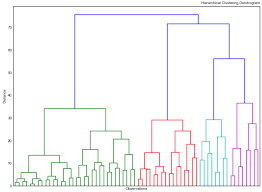
\includegraphics[width=8cm]{capitolo3/dendo.png}
	\centering
	\caption{Esempio di dendogramma}
	\label{fig:dendo}
\end{figure}


\subsection{Metodo basato sulle densità}

Questo metodo è in grado di individuare raggruppamenti di forme arbitrarie, inoltre permette una naturale protezione contro gli outlier. Questi algoritmi raggruppano gli oggetti in base a specifiche funzioni obiettivo di densità. La densità è solitamente definita come il numero di oggetti in un particolare quartiere di un insieme di dati. In questi approcci, un dato cluster continua a crescere finché il numero di oggetti nel quartiere supera un certo parametro.

Questi algoritmi possono essere di due tipi:
\begin{enumerate}
	\item Clustering della connettività basato sulla densità;
	\item Funzioni di densità Clustering;
\end{enumerate}

\subsection{Metodo delle partizioni}

I metodi di partizione danno generalmente come risultato un insieme di M cluster, in cui ogni oggetto appartiene a un gruppo.
Ogni cluster può essere rappresentato da un centroide, un vettore centrale, che non per forza è un elemento del dataset, o medoide, un elemento di un cluster la cui dissimilarità media rispetto a tutti gli oggetti nel cluster è minima. 
Ci sono diverse sistemi di partizionamento, a seguire verrà approfondito l'algoritmo di \textbf{K-mean} basato sull'utilizzo dei centroidi, che è il metodo utilizzato all'interno di questo lavoro, nonché uno dei metodi più popolari ed efficienti\cite{rai2010survey}.





\section{Algoritmo K-mean}

L'algoritmo di K-mean, anche noto come algoritmo di Lloyd, è un algoritmo iterativo che cerca di partizionare il dataset in K sottogruppi, predefiniti e non sovrapponibili, dove ogni punto appartiene ad un unico gruppo. 
\begin{algorithm}[h]
	\caption{Algoritmo del K-mean}
	Raggruppare i dati in $K$ gruppi, con $K$ predefinito;\\
	Per ogni cluster selezionare casualmente $K$ centri;\\
	Assegnare gli oggetti al centro del cluster più vicino in base alla funzione di distanza euclidea : $d(A,B) = \vert|(A,B)|\vert$ = $\sqrt{(a_1 - b_1)^2 + \dots + (a_n - b_n)^2}$, con $A,B \in \mathbb{R}^n$;\\
	Calcolare il centroide o la media di tutti gli oggetti di ciascun cluster;\\
	Ripetere i passaggi 2, 3 e 4 finché non converge.\\
	
\end{algorithm}

Cerca di rendere i punti di dati all'interno del cluster il più simili possibile, mantenendo al contempo i cluster il più possibile diversi (lontani).
L'algoritmo, in pratica, assegna i dati ad un cluster in modo tale che la somma della distanza al quadrato tra i punti e il centroide (media aritmetica di tutti i punti dati che appartengono a quel cluster) sia minima. Minore è la variazione all'interno dei cluster, più omogenei (simili) sono i punti di dati all'interno dello stesso.


L'approccio che segue il K-mean per risolvere il problema è chiamato \textbf{Expectation-Maximization} (EM).

Nello specifico il passo \textbf{E} consiste nell'assegnare i punti dati al cluster più vicino, mentre il passo \textbf{M} consiste nel calcolare il centroide di ciascun cluster. Di seguito viene illustrato il modo in cui si può risolvere matematicamente il problema.
La funzione obiettivo è:
\begin{align*}
	J = \sum_{i=1}^{m} \sum_{k=1}^{K} w_{ik} \vert|x_i - \mu_k|\vert
\end{align*}

dove $w_{ik}=1$ per il punto $x_i$ se appartiene al cluster $k$, altrimenti $w_{ik}=0$, mentre $\mu_k$ è il centroide del cluster di $x_i$.

Si tratta di un problema di minimizzazione composto da due parti. Prima si minimizza $J$ rispetto a $w_{ik}$ considerando $\mu_k$ fisso. Successivamente si minimizza $J$ rispetto a $\mu_k$ e si considera $w_{ik}$ fisso. Tecnicamente, prima si differenzia J rispetto a $w_{ik}$ aggiornando l'assegnazione dei cluster (passo E). Poi si differenzia J rispetto a $\mu_k$ e si ricalcolano i centroidi dopo le assegnazioni dei cluster del passo precedente (passo M). Pertanto, il passo E è:
\begin{align*}
	\frac{\delta J}{\delta w_{ik}} = \sum_{i=1}^{m} \sum_{k=1}^{K} \vert|x_i - \mu_k|\vert 
	\implies w_{ik} = \begin{cases}
		1, \text{se }  k=argmin_j \vert|x_i - \mu_k|\vert \\
		0, \text{altrimenti}
	\end{cases}
\end{align*}

In altre parole, si assegna $x_i$ al cluster più vicino, giudicato in base alla somma della distanza quadratica dal centroide del cluster.

Il passo M è:
\begin{align*}
\frac{\delta J}{\delta \mu_k} = 2\sum_{i=1}^{m} w_{ik}(x_i - \mu_k) = 0
\implies \mu_k = \frac{\sum_{i=1}^{m} w_{ik}x_i}{\sum_{i=1}^{m} w_{ik}}
\end{align*}

Il che si traduce nel ricompilare il centroide di ciascun cluster per riflettere le nuove assegnazioni.

Bisogna fare alcune precisazioni:
\begin{itemize}
	\item Poiché gli algoritmi di clustering, tra cui proprio il k-mean, utilizzano misure basate sulla distanza per determinare la somiglianza tra i dati, si raccomanda di standardizzare i dati in modo che abbiano una media pari a zero e una deviazione standard pari a uno, poiché quasi sempre le feature dei dataset hanno unità di misura diverse, ad esempio l'età o il dosaggio di un farmaco.
	\item Data la natura iterativa del K-mean e l'inizializzazione casuale dei centroidi, scelte diverse possono portare a cluster diversi, pertanto  l'algoritmo può rimanere bloccato in un ottimo locale e non convergere verso quello globale. Pertanto, si raccomanda di eseguire l'algoritmo utilizzando diverse inizializzazioni dei centroidi e di scegliere i risultati dell'esecuzione che ha prodotto la somma della distanza quadratica più bassa.
\end{itemize}

\subsection{Metriche per la scelta di $K$}

L'analisi di clustering non ha una solida metrica di valutazione che si può usare per misurare i risultati dei diversi algoritmi. Inoltre, poiché il K-mean richiede K come input e non lo apprende dai dati, non esiste una risposta giusta in termini di numero di cluster da avere in qualsiasi problema. 
A volte la conoscenza del dominio e l'intuizione possono aiutare, ma non è sempre così. Nella metodologia cluster-predict, si può valutare il rendimento dei modelli sulla base di diversi K cluster.
Tra le metriche possibili per valutare la scelta di K ve ne sono due:
\begin{itemize}
	\item Metodo Elbow
	\item Silhouette score
\end{itemize}
 
Nel dettaglio il silhouette score, quello sfruttato per questo lavoro, è utilizzato per determinare il grado di separazione tra i cluster.

Per ogni campione:
\begin{itemize}
	\item Calcola la distanza media di tutti i punti nello stesso cluster ($a_i$);
	\item Calcola la distanza media di tutti i punti al cluster più vicino ($b_i$);
	\item Calcola il coefficiente:
	\begin{align*}
		 \frac{b_i - a_i}{\max(a_i,b_i)}
	\end{align*}
\end{itemize}

Il coefficiente può avere valori nell'intervallo [-1,1]. 

$$\left \{
	\begin{array}{lc}
		1, & \text{i cluster sono molto distanti tra di loro}\\
		 0,  & \text{i cluster sono molto vicini tra di loro}\\
	   -1, & \text{i campioni sono assegnati ai cluster sbagliati}\\
	\end{array}
\right.
$$
\\
Per avere un buon cluster, l'obiettivo è avere il coefficiente più grande possibile e più vicino possibile a 1.

Spesso può essere utile applicare il K-mean su sottospazi dell'insieme originale. Tali sottoinsiemi vengono ottenuti a partire dal dataset originale con la trasformazione attraverso l'analisi delle componenti principali, nota come \textbf{PCA}.
\\

\section{PCA}

La PCA è una tecnica che è largamente usata in applicazioni quali riduzione delle dimensioni, compressione dei dati, estrazione delle feature e visualizzazione dati.\\
Ci sono due definizioni che si risolvono nel medesimo algoritmo, ossia la PCA può essere definita come la proiezione ortogonale dei dati in uno spazio lineare di dimensioni inferiori, noto come il sottospazio principale, tale che la varianza dei dati proiettati sia massimizzata.\\ Equivalentemente può essere definita come la proiezione lineare che minimizza il costo medio della proiezioni, ossia la distanza quadratica media tra i punti e la loro proiezione\cite{bishop2006pattern}.

L'algoritmo di PCA ha le seguenti fasi:
\newpage
\begin{algorithm}[h]
	\caption{Algoritmo di PCA}
	Standardizza i dati;\\
	Calcola la matrice di covarianza; \\
	Calcola gli autovettori e gli autovalori a partire della matrice di covarianza;\\
	Seleziona le prime k componenti principali che catturano la massima quantità di varianza;\\
	Proietta i dati sulle componenti principali.
	\label{alg:PCA}
\end{algorithm}

Il valore delle k componenti viene deciso in precedenza e al passo 5 dell'algoritmo per trasformare i dati nello spazio sottodimensionato definito dalle componenti principali si moltiplica semplicemente il dato normalizzato per la componente principale.


\subsection{Interpretazione matematica}

Per comprendere a pieno la PCA e come vengono determinate le componenti principali, è importante comprendere l'aspetto matematico che si trova alla base.

Il primo concetto da definire è quello di matrice di covarianza. 
La varianza e la covarianza rappresentano lo "\textit{spread}" di un insieme di punti intorno al loro centro (media).
La covarianza è misurata tra due valori per determinare se ci sia una relazione tra di loro.
A seguire la formula della covarianza tra $X$ e $Y$:
\begin{equation*}
	cov_{XY} = \frac{\sum_{i=0}^{N-1} (x_1 - \bar{x})(y_i - \bar{y})}{N-1}
\end{equation*}
dove $\bar{x}$ e $\bar{y}$ rappresentano la media per $X$ e $Y$ rispettivamente. 
In generale, $cov_{XX} = var_X$, infatti:
\begin{equation*}
	cov_{XX} = \frac{\sum_{i=0}^{N-1}(x_1 - \bar{x})(x_i - \bar{x})}{N-1} = \frac{\sum_{i=0}^{N-1} (x_1 - \bar{x})^2}{N-1} = var_X
\end{equation*}

La matrice di covarianza $C$ dei vettori $X_1, X_2, \dots , X_n $ è definita come la matrice quadrata $C\in \mathbb{R}^{n \times n}$ ,tale che:

\begin{equation*}
	C= \begin{pmatrix}
		var_{X_1} & cov_{X_1,X_2} & \dots & cov_{X_1,X_n}\\ 
		cov_{X_2,X_1} & var_{X_2} & \dots & cov_{X_2,X_n}\\
		\vdots & \vdots & \ddots & \vdots \\
		cov_{X_n,X_1} &  cov_{X_n,X_2} & \dots & var_{X_n}\\
	\end{pmatrix}
\end{equation*}
\newline
La covarianza è simmetrica, ossia $cov_{X,Y} = cov_{Y,X}$ pertanto anche la matrice di covarianza sarà simmetrica rispetto la diagonale principale.

Dalla matrice delle covarianze è facilmente possibile calcolare gli autovettori e autovalori. Intuitivamente un autovettore è un vettore le cui dimensioni restano invariate quando gli viene applicata una trasformazioni lineare.
Gli autovalori di C sono le radici $\lambda$ dell'equazione caratteristica :
\begin{equation*}
	det(C - \lambda I) = 0
\end{equation*}

$I$ rappresenta la matrice identità di dimensioni $n \times n$.
A partire da questi autovalori $\lambda_1, \dots, \lambda_n$ saranno poi ottenuti i corrispondenti autovettori $v_i$ con $ i \in [1,n]$, che successivamente saranno ordinati in maniera decrescente rispetto il corrispondente autovalore da cui si generano, perciò si avra $ v_1  \geq v_2 \geq \dots \geq v_n$

Gli autovettori rappresentano proprio le Componenti Principali:

\begin{equation*}
	v_1 = \begin{bmatrix}
					\phi_{11}\\
					\phi_{21}\\
					\vdots\\
					\phi_{n1}
				\end{bmatrix},
	v_2 = \begin{bmatrix}
					\phi_{12}\\
					\phi_{22}\\
					\vdots\\
					\phi_{n2}
				\end{bmatrix},
	\dots ,
	v_n = \begin{bmatrix}
					\phi_{1n}\\
					\phi_{2n}\\
					\vdots\\
					\phi_{nn}
			   \end{bmatrix}
\end{equation*}
\newline
Gli elementi  $\phi_{ij}$ con $i,j =1, \dots ,n$ sono i loadings delle componenti principale. Per calcolare i loadings si deve trovare il vettore $\phi$ che massimizza la varianza.
Tramite tecniche di algebra lineare si può mostrare che l'autovettore corrispondente al più grande autovalore della matrice di covarianza è l'insieme dei loadings che spiegano la più grande proporzione della variabilità.
Ogni vettore delle componenti principali definisce una direzione nello spazio delle feature, poiché gli autovettori sono ortogonali tra di loro, i loadings e perciò le componenti principali non sono correlate tra di loro e formano le basi del nuovo spazio.

Come detto in precedenza lo scopo della PCA è ridurre la dimensionalità cercando di spiegare la maggior parte di varianza possibile.
La proporzione di varianza spiegata (\textbf{PVE}) dell'$i$-esima componente principale è definita come: 
\begin{equation*}
	PVE = \frac{\lambda_i}{\sum_{j=1}^{n} \lambda_j}
\end{equation*}
Ossia il PVE è calcolato semplicemente dalla componente principale $i$ prendendo l'$i$-esimo autovalore e dividendolo per la somma di tutti gli autovalori.

\section{PCA e K-Mean}
La PCA può aiutare la clusterizzazione tramite K-mean in diversi modi:
\begin{enumerate}
	\item Riduzione delle dimensioni: la PCA può essere utilizzata per ridurre la dimensionalità dei dati prima di applicare l'algoritmo di K-mean. Riducendo le dimensioni, si aiuta nella rimuzione di rumori e di feature irrilevanti così da migliorare le performance sul clustering.
	\item La PCA può aiutare a migliorare le performance riducendo la complessità computazionale dell'algoritmo con minori dimensioni il K-mean può lavorare in maniera più efficiente portando a risultati di clusterizzazione più veloci.
	\item Visualizzazione: la PCA può aiutare nella visualizzazione dei dati in uno spazio sottodimensionato riducendo le dimensioni a due o tre componenti è possibile plottare i dati su un grafo che permette una migliore identificazione di cluster e modelli sui dati.
	
\end{enumerate}

\section{Caso di studio}

In questa sezione verranno mostrati e analizzati i risultati ottenuti applicando PCA e K-mean su una parte del dataset ottenuto dal registro ARRT, descritto in precedenza.
Più nel dettaglio l'obiettivo che questo lavoro si pone è determinare l'esistenza di un modello di clusterizzazione dei pazienti. L'analisi è basata esclusivamente sui dati clinici e  le misurazioni sono ristrette ai valori registrati nel monitoraggio al tempo 0. Sono state escluse, inoltre, le feature relative agli score (SOFA Score, Apachi Score e SAP Score), questi valori saranno successivamente utilizzati, insieme ai dati sulle mortalità, per verificare la validià dei risultati ottenute. Per queste analisi, in accordo con i medici coinvolti nel progetto, si ristringe a 175 il numero di pazienti considerati, che rappresentano l'insieme di pazienti con i dati più completi, va ricordato, infatti, che il registro è tutt'ora attivo e i dati possono essere ancora inseriti o modificati. Pertanto il dataset utilizzato in questa fase si compone di 175 righe per 148 colonne.

La prima tecnica che si incontra è la PCA, che come già detto in precedenza ha diverse utilità. Uno degli scopi per cui è stata utilizzata è senza dubbio per ridurre le dimensioni delle feature, permettendo,così, una visualizzazione dei dati su dimensioni ridotte.

Ovviamente il primo passo è stato quello di normalizzazione dei dati. La tecnica scelta è il \textit{MinMaxScaler}, che trasforma le feature scalandole ognuna individualmente rispetto un intervallo dato, lo standard è $[0,1]$, ma può essere modificato.  La trasformazione è la seguente:
\begin{equation*}
	X_{scalato} = \frac{x-x_{min}}{x_{max} - x_{min}} 
\end{equation*}
Dove $x_{max}$ e $x_{min}$ rappresentano il valore massimo e minimo rispettivamente della feature analizzata.

L'obiettivo da raggiungere applicando la PCA è quello di salvaguardare il maggior numero di varianza riducendo le feature. 
\begin{figure}[h]
	\begin{subfigure}{.5\textwidth}
		\centering
		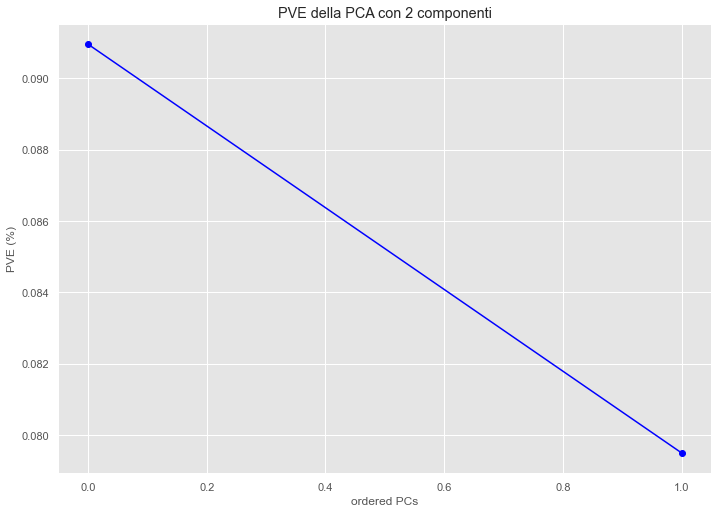
\includegraphics[width=.5\linewidth]{capitolo3/pca.png}
		\caption{PVE della PCA con 2 componenti}
		\label{fig:pca2d}
	\end{subfigure}%
	\begin{subfigure}{.5\textwidth}
		\centering
		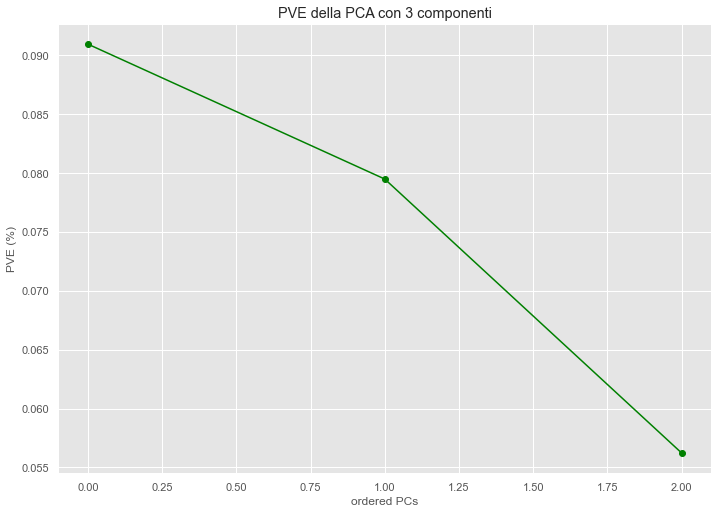
\includegraphics[width=.5\linewidth]{capitolo3/pca_3.png}
		\caption{PVE della PCA con 3 componenti}
		\label{fig:pca3d}
	\end{subfigure}
	\caption{PVE della PCA con 2 e 3 componenti}
	\label{fig:pca}
\end{figure}
Applicando il modello e cercando di garantire una percentuale di varianza all'80\%  si otterrebbe un numero di 32 componenti, certamente ci sarebbe una dimuzione netta dei rappresentanti, ma non sufficiente per permettere una visualizzazione dei dati efficiente. Per questo motivo si valutano i valori della varianza PCA con 2 e 3 componenti.\\
Come si può vedere dalla figura \ref{fig:pca} nella PCA con 3 componenti (figura \ref{fig:pca3d}) si riesce, come prevedibile, ad avere una percentuale di varianza maggiore.
Nel dettaglio si ha che la varianza percentuale totale con 2 componenti è del 17\% che raggiunge circa il 23\% nel caso con 3. Visto il miglior risultato utilizzando 3 dimensioni le considerazioni a seguire verranno applicate rispetto a quel modello.

Sono state individuate le feature che maggiormente influiscono sulle componenti principali, questo per aiutare un'analisi medica a posteriori sui risultati ottenuti (figure \ref{fig:comp1},\ref{fig:comp2} e \ref{fig:comp3})

\begin{figure}  
	\begin{minipage}{0.45\textwidth} 
		\centering
		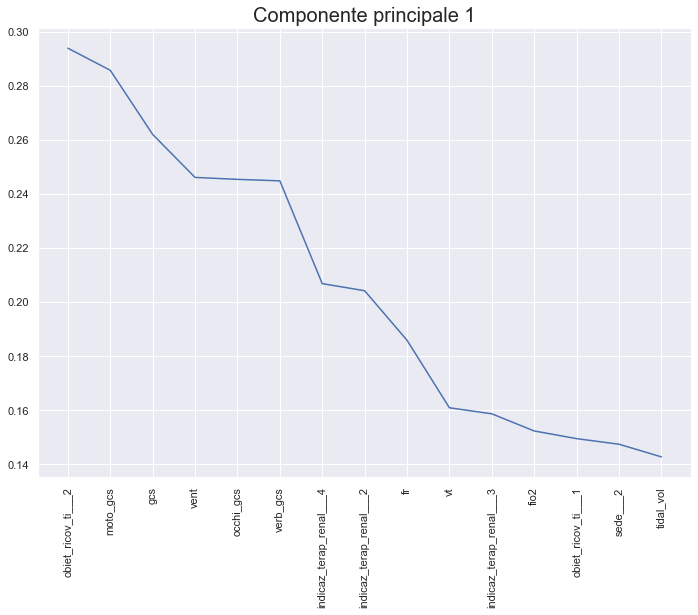
\includegraphics[width=6cm]{capitolo3/comp1.png}
		\caption{Feature ordinate rispetto la prima componente principale}
		\label{fig:comp1}  
	\end{minipage}    
	\hspace{\fill}  %% no blank line before of after this instruction
	\begin{minipage}{0.45\textwidth} 
		\centering
		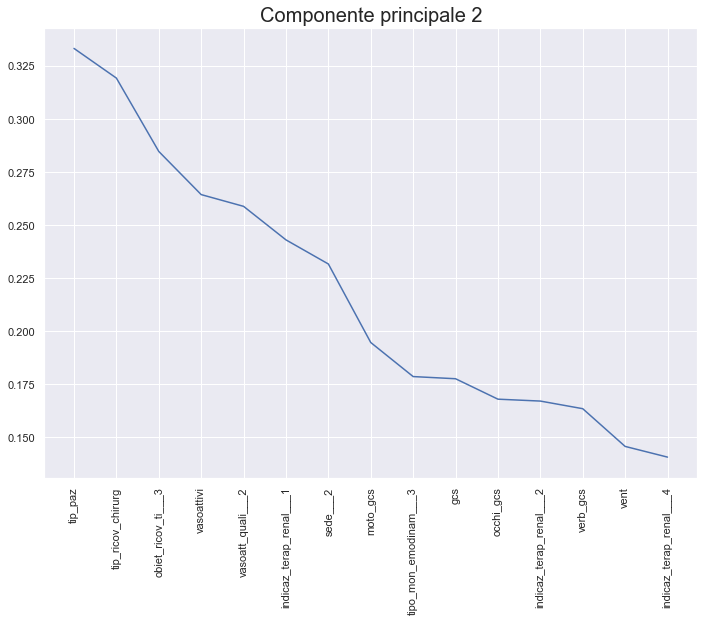
\includegraphics[width=6cm]{capitolo3/comp2.png}
		\caption{Feature ordinate rispetto la secionda componente principale}
		\label{fig:comp2}  
	\end{minipage}    
	
	\vspace{0.75cm}
	\centering
	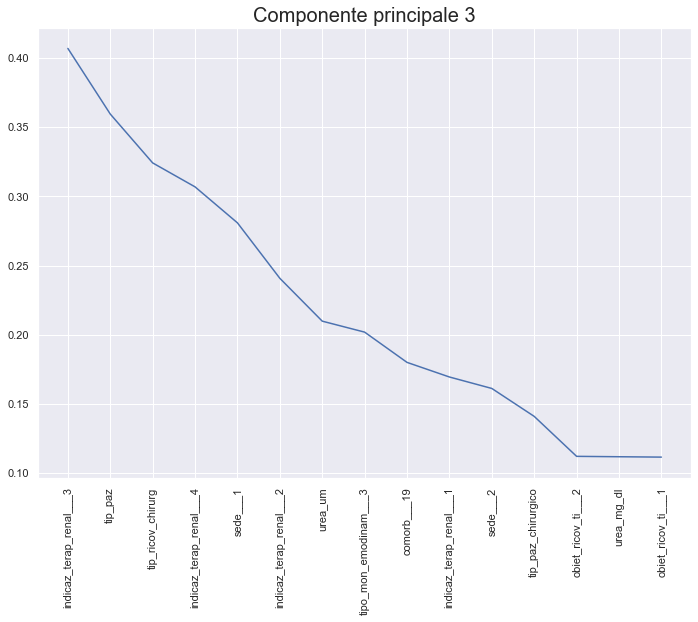
\includegraphics[width=6cm]{capitolo3/comp3.png}
	\caption{Feature ordinate rispetto la terza componente principale}
	\label{fig:comp3} 
  
\end{figure}



Per concludere le analisi sulla PCA, il modello è stato applicato sugli score e sulla mortalità, entrambi vengono indagati rispetto i monitoraggi dal momento di ingresso al giorno 3.
Da queste analisi il risultato ottenuto mostra un evidente suddivisione dei pazienti in due gruppi. Come evidenziato dalla figura \ref{fig:esiti} si nota a sinistra un gruppo certamente più numeroso e fitto, rispetto ad un gruppo sulla destra più ristretto. In questo secondo gruppo oltre ad evidenziarsi una mortalità sui 3 giorni inferiore, si nota anche un valore medio del SOFA score più basso (figura \ref{fig:sofa}).

\begin{figure}[h]
	\centering
	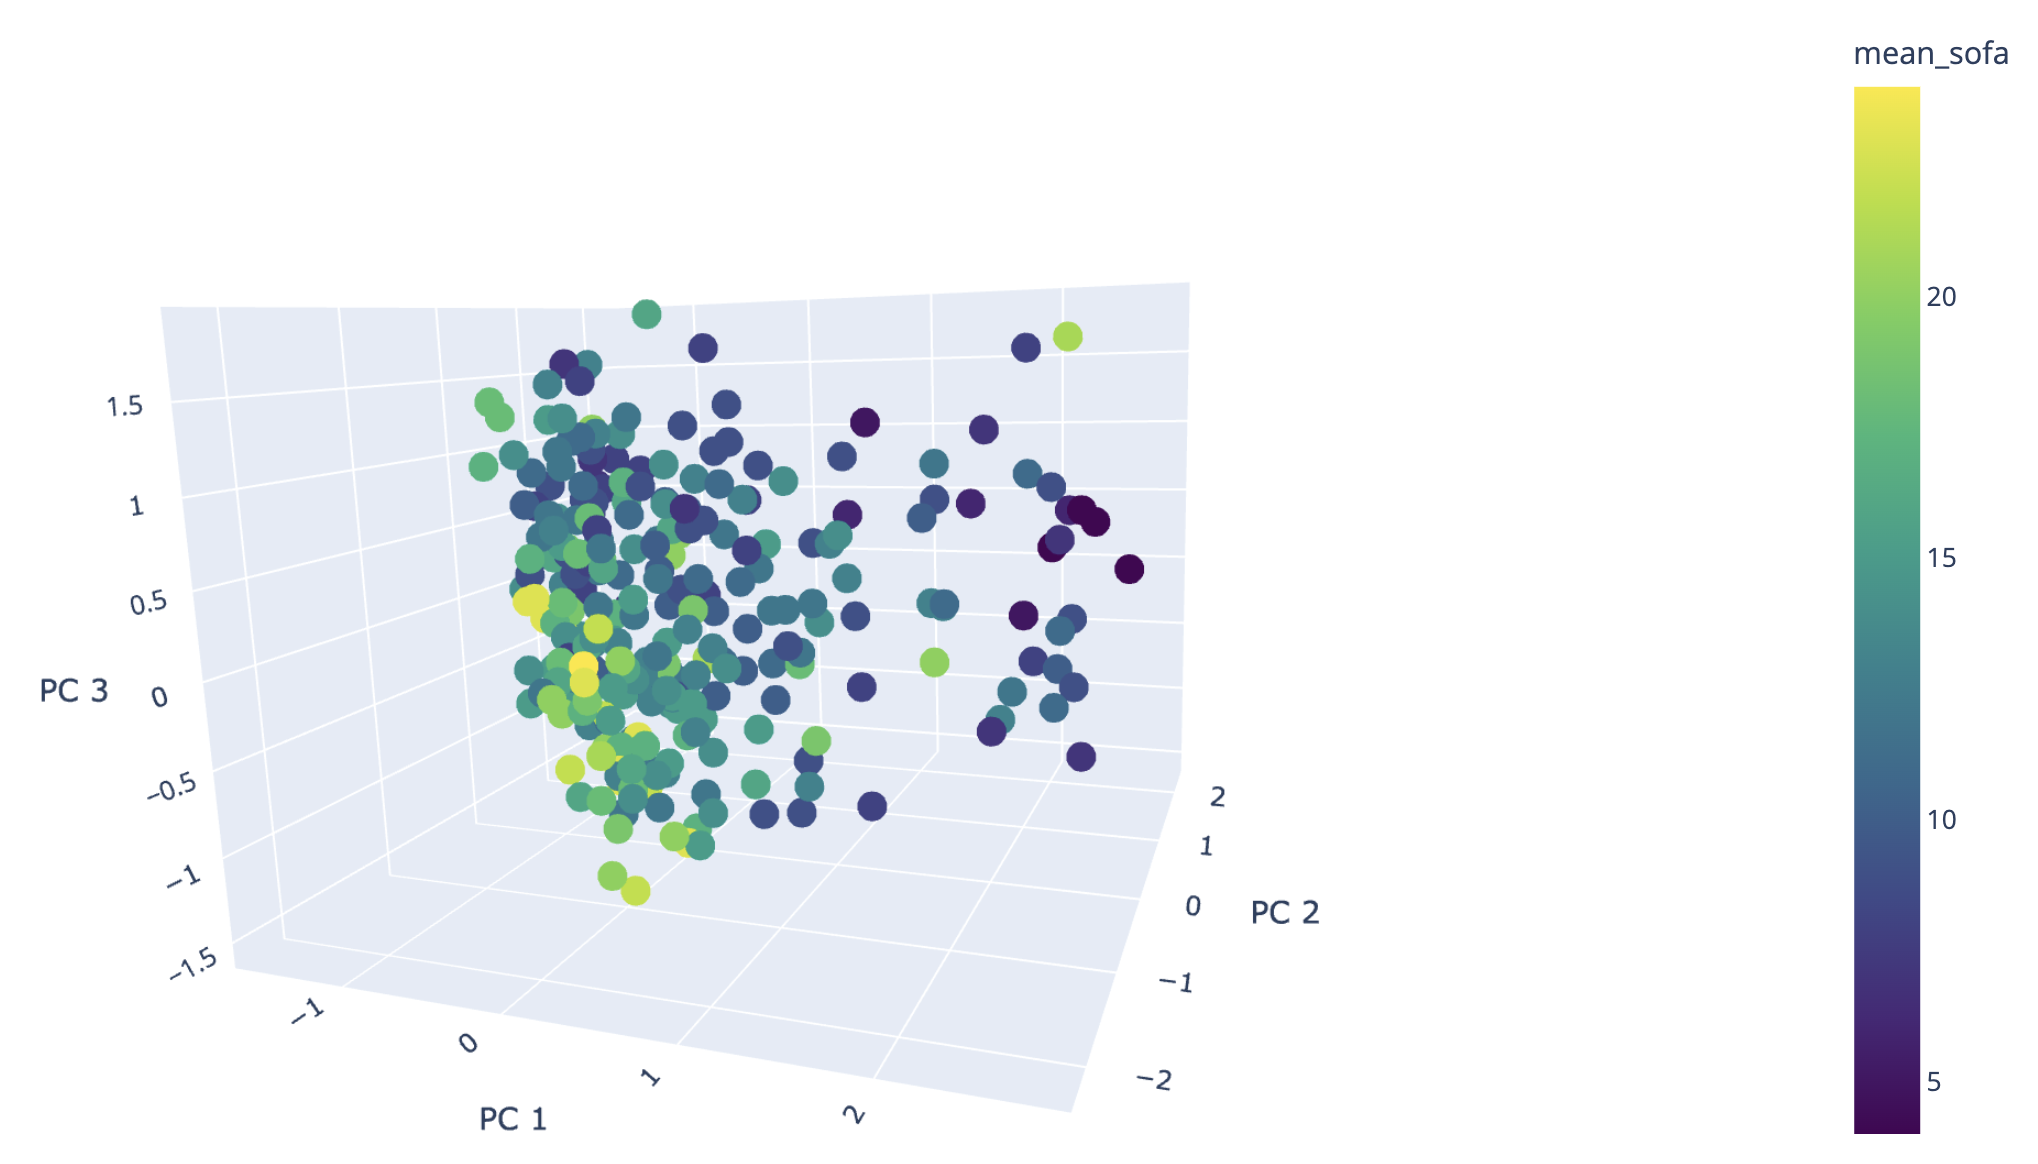
\includegraphics[width=12cm]{capitolo3/sofa.png}
	\caption{Sofa Score medio visualizzato rispetto al modello della PCA}
	\label{fig:sofa}
\end{figure}
\begin{figure}[h]
	\centering
	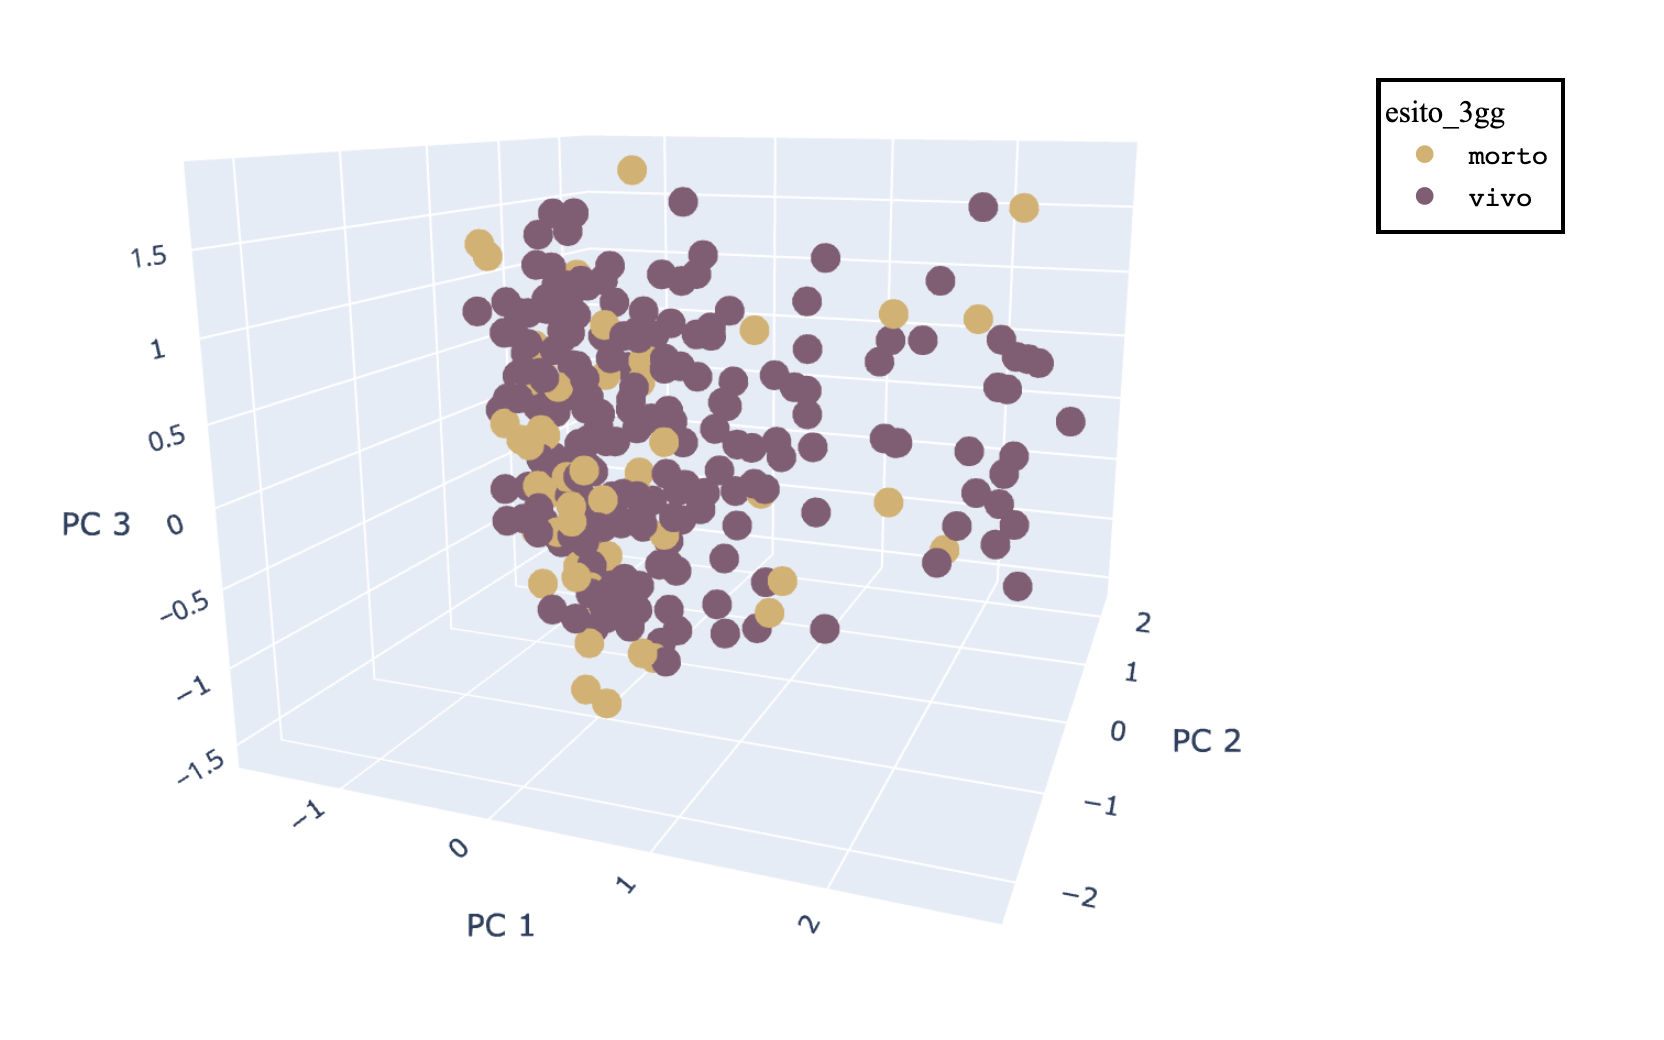
\includegraphics[width=12cm]{capitolo3/esiti.png}
	\caption{Esito della mortalità sui 3 giorni applicato sul modello di PCA}
	\label{fig:esiti}
\end{figure}

Sulla base di quanto ottenuto fin qui si è proceduto ad applicare l'algoritmo di clustering del K-mean per verificare che i risultati ottenuti rispecchino l'andamento dei dati.
Per la scelta del valore di K vengono considerati i risultati del silhouette score per K=2 e K=3, il numero di iterazioni viene posto a 10, ottenendo così una convergenza sul modello.
\begin{figure}  
	\begin{minipage}{0.5\textwidth} 
		\centering
		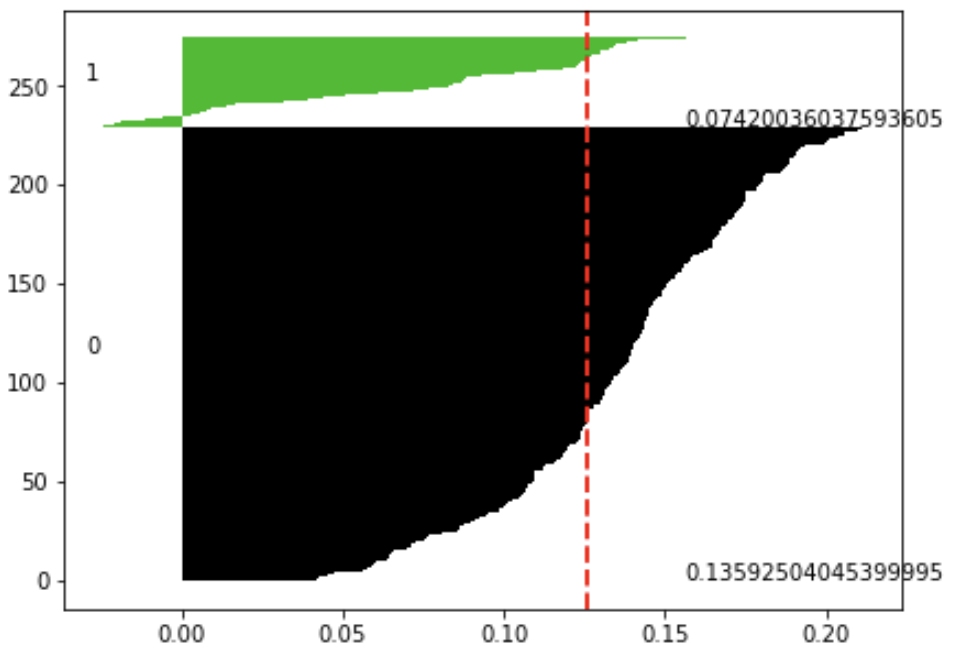
\includegraphics[width=6cm]{capitolo3/sil2.png}
		\caption{Silhouette score per K=2}
		\label{fig:sil1}  
	\end{minipage}    
	\hspace{\fill}  %% no blank line before of after this instruction
	\begin{minipage}{0.5\textwidth} 
		\centering
		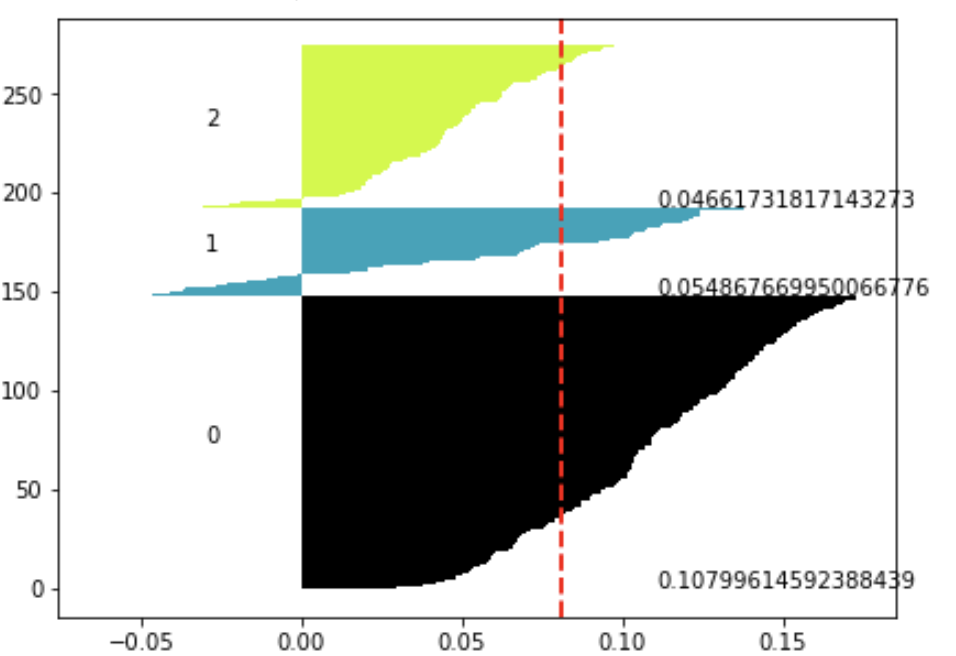
\includegraphics[width=6cm]{capitolo3/sil3.png}
		\caption{FSilhouette score per K=3}
		\label{fig:sil2}  
	\end{minipage}    
\end{figure}

Mettendo a confronto gli score si ottiene un risultato migliore per K=2 (figura \ref{fig:sil1}) che se rappresentato sullo spazio sottodimensionato ottenuto con il PCA a 3 componenti, rispetta l'andamento ottenuto nelle precedenti valutazioni (figura \ref{fig:kmean}).

\begin{figure}[h]
	\centering
	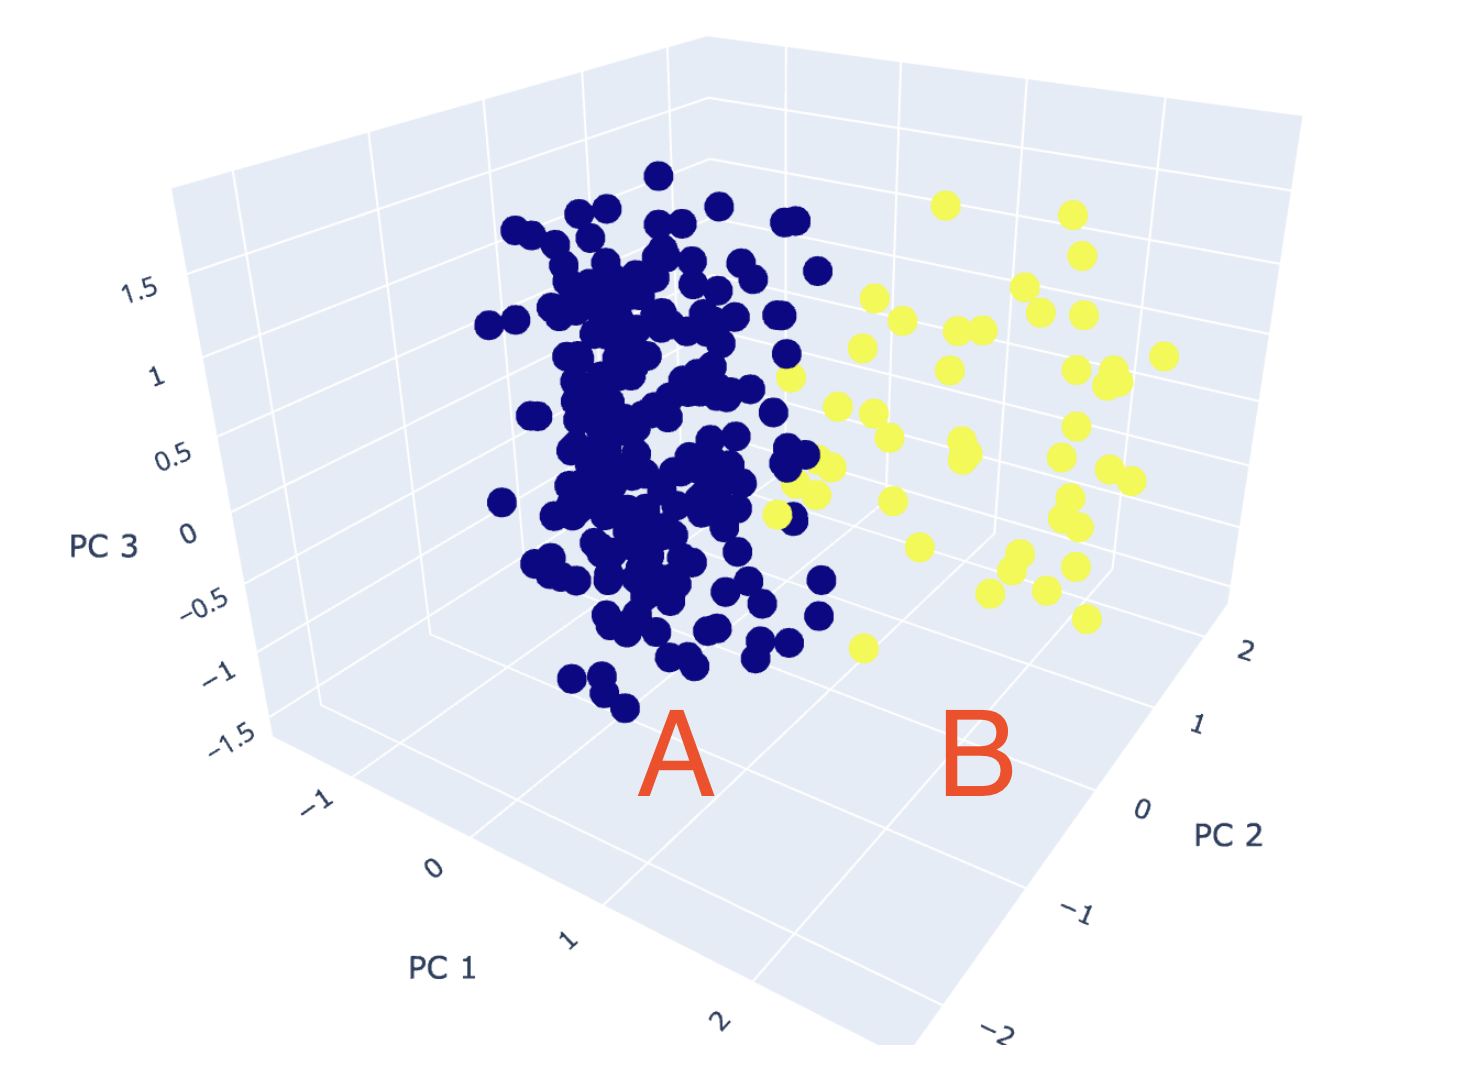
\includegraphics[width=14cm]{capitolo3/kmean.png}
	\caption{Clustering applicato sullo spazio sottodimensionato ottenuto con la PCA, i due cluster vengono indicati rispettivamente con A e B. }
	\label{fig:kmean}
\end{figure}

\newpage
In conclusione sono state eseguite delle ulteriori analisi sui due cluster A e B separatamente.
Nella tabella \ref{table:cluster1} sono illustrati le percentuali di mortalità per i due cluster rispetto gli archi temporali.

\begin{table}[h!]

	\parbox{.45\textwidth}{
	\centering
	\begin{tabular}{ |c| c|c|} 
		\hline
		\multicolumn{3}{|c|}{Percentuale di mortalità su A} \\
		\hline
		\textbf{Tempo} & \textbf{Vivi} & \textbf{Morti} \\
		\hline
		\hline
		12 ore & 97\% & 3\% \\
		\hline
		24 ore & 90\% & 10\% \\
		\hline 
		2 giorni & 85\% & 15\% \\
		\hline
		3 giorni & 79\% & 21\% \\
		\hline
	\end{tabular}}
	\quad
	\parbox{.45\textwidth}{
		\centering
		\begin{tabular}{ |c| c|c|} 
			\hline
			\multicolumn{3}{|c|}{Percentuale di mortalità su B} \\
			\hline
			\textbf{Tempo} & \textbf{Vivi} & \textbf{Morti} \\
			\hline
			\hline
			12 ore & 100\% & 0\% \\
			\hline
			24 ore & 98\% & 2\% \\
			\hline 
			2 giorni & 96\% & 4\% \\
			\hline
			3 giorni & 87\% & 13\% \\
			\hline
	\end{tabular}}
	\caption{Percentuale di mortalità per i due cluster}
	\label{table:cluster1}
\end{table}

Un'analisi simile si esegue anche rispetto ai valori del SOFA score (tabella \ref{table:cluster2}) al tempo 0 suddividendo i valori in 3 gruppi: 
\begin{itemize}
	\item Gruppo 1 : valori inferiori a 7;
	\item Gruppo 2: valori compresi tra 7 e 14;
	\item Gruppo 3: valori superiori al 14;
\end{itemize}

\begin{table}[h!]
	
	\parbox{.50\textwidth}{
		\centering
		\begin{tabular}{ |c| c|} 
			\hline
			\multicolumn{2}{|c|}{Percentuali SOFA score su A} \\
			\hline
			\textbf{Gruppo} & \textbf{Percentuale pazienti}\\
			\hline
			\hline
			Gruppo 1 & 3\% \\
			\hline
			Gruppo 2& 56\%  \\
			\hline 
			Gruppo 3 & 41\% \\
			\hline
	\end{tabular}}
	\quad
	\parbox{.50\textwidth}{
		\centering
		\begin{tabular}{ |c| c|} 
			\hline
			\multicolumn{2}{|c|}{Percentuali SOFA score su B}  \\
			\hline
			\textbf{Gruppo} & \textbf{Percentuale pazienti} \\
			\hline
			\hline
			Gruppo 1 & 31\% \\
			\hline
			Gruppo 2& 58\%  \\
			\hline 
			Gruppo 3 & 11\% \\
			\hline
	\end{tabular}}
	\caption{Percentuale di SOFA score per i due cluster}
	\label{table:cluster2}
\end{table}